

\section{Diseño}
\label{sec:diseno}

Diseño
QUE BUSCAMOS
La finalidad de nuestra aplicación es poder generar scripts completamente funcionales, que sean capaz de manejar con éxito un robot de características complejas, a partir de un proyecto del lenguaje de programación visual Scratch 2.0

DIVISION DEL PROBLEMA

PIEZAS PRINCIPALES

--extensión en scratch

--traducción de scratch

--aplicación sobre el robot real

ESQUEMA DE LAS PIEZAS EN CONJUNTO

EXPLICACION DEL FUNCIONAMIENTO EN CONJUNTO

--esto se comunica con lo otro, traduce de esta forma(cosas del script de traducción), el python traducido se ejecuta, estableciendo la comunicación con el simuladior o el robot real de tal forma.
\section{kurt}
\label{sec:kurt}

Kurt es una biblioteca de Python que permite la manipulación compleja de proyectos Scratch (archivos .sb o .sb2) a través de simples comandos de Python. Incluye un decompilador, que permite que un proyecto se cargue en un conjunto de objetos de Python, y un compilador que permite el empaquetamiento de un conjunto de scripts de imágenes / texto en proyectos scratch.

Vamos a estudiar más a fondo como trabaja con esta librería.


\subsection{Traduccion con kurt}
\label{sec:traduccion}
La clase principal de kurt almacena el contenido de un archivo de proyecto Scratch.
Los contenidos incluyen variables globales y listas, el escenario y los sprites, cada uno con sus propios scripts, sonidos, variables y listas.
\begin{lstlisting}[language=python,firstnumber=1]
# load the scratch project
p = kurt.Project.load(open_path + sys.argv[1])

# show the blocks included
for scriptable in p.sprites + [p.stage]:
	for script in scriptable.scripts:
		# exclude definition scripts
		if "define" not in script.blocks[0].stringify():
			s = script
print("Stringify:")
sentences = []
for b in s.blocks:
	print(b.stringify())
\end{lstlisting}
traduccion con kurt

\section{Desarrollo de bloques}
\label{sec:desarrollo-de-bloques}

Scratch facilita el uso de bloques personalizados mediante extensiones externas, estas  extensiones externas a la aplicación se definen mediante el uso de ficheros JSON, aunque por convención, en Scratch tentrán extensión .s2e .

Este tipo de ficheros se creó para la comunicación mediante HTTP de bloques con aplicaciones auxiliares, por ejemplo algún tipo de hardware.
Un \textit{AppHelper} se ejecuta en segundo plano, lista para ser utilizada por los proyectos de Scratch que usan esa extensión.
Cada extensión tiene un número de puerto único. Scratch busca la aplicación de ayuda en el número de puerto dado en la máquina local.
Se comunica con el \textit{AppHelper} utilizando el protocolo HTTP, la aplicación envía comandos al \textit{AppHelper} y este envía los valores del sensor y la información de estado a Scratch a través de solicitudes HTTP GET. Dado que el protocolo es HTTP estándar, cualquier navegador se puede usar para probar y depurar aplicaciones de ayuda.

Pero nostros no vamos a utilzar esta funcionalidad, únicamente nos ayudamos de éste documento .s2e para definir nuestra extensión y pueda ser usada desde el IDE offline de scratch.

El objeto JSON en el archivo de descripción de la extensión incluye el nombre de la extensión, el puerto TCP / IP utilizado para comunicarse con el \textit{AppHelper} y una lista de bloques de Scratch.
\begin{lstlisting}[language=json,firstnumber=1]
{ 
  "extensionName": "Extension Example",
  "extensionPort": 12345,
  "blockSpecs": [
    [" ", "beep", "playBeep"],
	[" ", "set beep volume to %n", "setVolume", 5],
	["r", "beep volume", "volume"],
  ]
}
\end{lstlisting}
El nombre de esta extensión es "Ejemplo de extensión" y se conecta a su aplicación auxiliar en el puerto 12345. El
El campo "blockSpecs" describe los bloques de extensión que aparecerán en el apartado "Más bloques" en la aplicación de Scratch.
En en este caso, hay tres bloques: (1) un bloque de comandos que reproduce un pitido; (2) un bloque de comando que
establece el volumen del pitido; y (3) un bloque que devuelve un valor, que informa del volumen de un pitido.


Cada bloque se describe mediante una matriz con los siguientes campos:
\begin{itemize}
\item \textbf{Tipo de bloque}:
\begin{itemize}
\item ' ' - bloque de comandos
\item 'w' - bloque de comandos que esperan
\item 'r' - bloque que retorna un valor
\item 'b' - bloque que retorna un booleano 
\end{itemize}
\item \textbf{Formato de bloque}

El formato de bloque es una cadena que describe las etiquetas y ranuras de parámetros que aparecen en el bloque.
Las ranuras de parámetros están indicadas por una palabra que comienza con '\%' y puede ser una de:
\begin{itemize}
\item \%n -  parámetro de número 
\item \%s - parámetro de cadena 
\item \%b - parámetro booleano
\end{itemize}
\item \textbf{Operación o nombre de variable remota}:
El campo de operación en una especificación de bloque se usa de dos maneras. Para bloques de comandos, se envía a la aplicación auxiliar, junto con cualquier valor de parámetro, para invocar una operación. O para retornar bloques, es el nombre de una variable de sensor. Los valores de la variable del sensor se guardan en un diccionario.
La ejecución de un bloque simplemente devuelve el valor reportado más recientemente para esa variable de sensor.
\item \textbf{(opcional) cero o más valores de parámetros predeterminados}

\item \textbf{Menus desplegables}:
Los bloques que definimos pueden hacer uso de parámetros de menú, los cuales definiremos de dos formas:
\begin{itemize}
\item \%m.menuName - parámetro de menú (no editable), proporciona un sencillo espacio para los parámetros del menú desplegable.
\item \%d.menuName - parámetro de número editable con menú, proporciona una ranura de parámetro numérico con un menú auxiliar.
\end{itemize}
\end{itemize}

Con todo esto podemos entender la definición de alguno de nuestros bloques como podemos en el siguiente extracto de código.
\begin{nobreak} 
\begin{lstlisting}[language=json,firstnumber=1]
{
  "extensionName": "Scratch4Robots",
  "extensionPort": 12345, 
  "blockSpecs": [
    ["", "stop robot-drone", "stop"],         
    ["", "move robot %m.robotDirections speed %n", "robot/move/speed", "forward", 1],
    ["r", "color detection %m.color", "camera/all","red"],
    ["r", "frontal laser distance", "laser/frontal"],
  ],
  "menus": {
    "robotDirections": ["forward", "back"],         
    "color": ["red", "blue"]
  }
}

\end{lstlisting}
\end{nobreak} 

\subsection{Bloques genericos}

\begin{figure}[H]
	\begin{minipage}{0.33\textwidth}
    	\centering
    	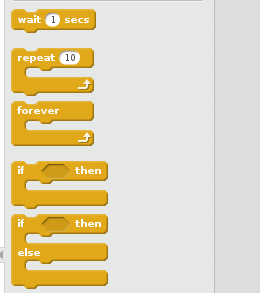
\includegraphics[scale=0.40]{img/bloques-control.png}
     	\caption{Bloques de control}
  		\label{fig:bloques-control}
   	\end{minipage}\hfill
   	\begin {minipage}{0.33\textwidth}
     	\centering
     	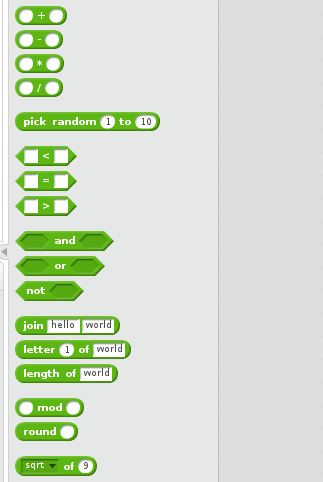
\includegraphics[scale=0.40]{img/bloques-mat.png}
  		\caption{Bloques matemáticos}
  		\label{fig:bloques-mat}
	\end{minipage}
	\begin {minipage}{0.33\textwidth}
     	\centering
     	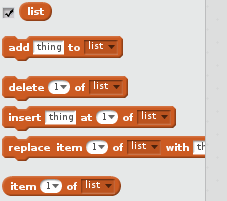
\includegraphics[scale=0.40]{img/bloques-listas.png}
     	\caption{Bloques de listas}
     	\label{fig:bloques-listas}
	\end{minipage}
\end{figure}
\begin{itemize}
\item \textbf{Bloques de operaciones matemáticas}
	\begin{itemize}

    \item \textbf{sqrt of ()}: Realiza la operación raiz cuadrada de un número dado
    \item \textbf{sin of ()}: Realiza la operación seno de un número dado
    \item \textbf{cos of ()}: Realiza la operación coseno de un número dado
    \item \textbf{tan of ()}: Realiza la operación tangente de un número dado
    \item \textbf{asin of ()}: Realiza la operación arcoseno de un número dado
    \item \textbf{acos of ()}: Realiza la operación arcocoseno de un número dado
    \item \textbf{atan of()}: Realiza la operación arcotangente de un número dado
    \item \textbf{log of ()}: Realiza la operación logaritmo de un número dado
    \item \textbf{ln of ()}: Realiza la operación logaritno neperiano de un número dado
    \item \textbf{abs of ()}: Devuelve el valor absoluto de un número
    \item \textbf{mod of ()}: Devuelve el módulo de un número dado
    \end{itemize}

\item \textbf{Bloques de operaciones lógicas}
\begin{itemize}

 \item \textbf{And}
 \item \textbf{Or}
 \item \textbf{NOT}
 \item \textbf{Mayor que}
 \item \textbf{Menor que}

\end{itemize}

\item \textbf{Bloques de control}
\begin{itemize}
\item \textbf{Wait () secs}: Pausa la ejecución el tiempo especificado, equivalente a la sentencia \textit{time.sleep()} de python.
\item \textbf{Forever}: Bucle infinito, equivalente a \textit{while(True)} en lenguaje python.
\item \textbf{If () then}: Comprueba la condición para que si la condición es verdadera, los bloques dentro de ella se ejecuten.
\item \textbf{If () Then, Else}: Comprueba la condición para que si la condición es verdadera, los bloques dentro de la primera condición se activen y si la condición es falsa, los bloques dentro de la segunda condición se activarán.
\item \textbf{Repeat ()}: Un ciclo que repite la cantidad de veces especificada, sería la equivalencia al bucle \textit{for} en python.
\end{itemize}
\item \textbf{Miscelaneos}
\begin{itemize}

\item \textbf{say ()}: Imprime lo que le añadas como argumento, equivalente  \textit{print}
\item \textbf{Set () to ()}: Utilizado para dar valor a una variable en concreto
\end{itemize}

\item \textbf{Bloques de listas}
\begin{itemize}

\item \textbf{Insert () at () of ()}: Inserta elemento en la posición seleccionada de la lista indicada.
\item \textbf{Item () of ()}: Devuelve el elemento almacenado en la posición indicada de la lista.
\item \textbf{Add () to ()}: Inserta en la listaInsert.
\item \textbf{Delete () of ()}: Elimina el elemento en una posición determinada de la lista.
\end{itemize}
\end{itemize}

\subsection{Bloques de drone}
\begin{itemize}
\item \textbf{Bloques perceptivos}
	\begin{itemize}
	\item \textbf{Pose3D}: Obtiene el valor de la posición 3D del robot
	\item \textbf{Color detection}: Haciendo uso de una cámara en el robot, detecta objetos de un determinado color, devolviendo su posición en la imagen.
	\end{itemize}
\item \textbf{Bloques de movimiento}
	\begin{itemize}
	\item \textbf{stop robot}: Pone a su valor inicial todas las velocidades del robot
	\item \textbf{drone take off} Makes the drone take off
	\item \textbf{drone land} Makes the drone land
	\item \textbf{drone move direction}: (forward, back, up, down, left, right), speed: velocity (integer)	Gives the drone a speed in the indicated direction
	\item \textbf{drone turn direction}: (left, right), speed: velocity (integer)		Gives the drone a turning speed in the indicated direction
	\end{itemize}
\end{itemize}



\subsection{robots con ruedas}
\begin{itemize}
\item \textbf{Bloques perceptivos}
	\begin{itemize}
	\item \textbf{Pose3D} :Obtiene el valor de la posición 3D del robot.
	\item \textbf{Color detection}: Haciendo uso de una cámara en el robot, detecta objetos de un determinado color, devolviendo su posición en la imagen.
	\item \textbf{Frontal distance}: Obtiene la medida promedio de los datos del láser frontal. 
	\end{itemize}
\item \textbf{Bloques de movimiento}
	\begin{itemize}

	\item \textbf{robot move ()}: Da una velocidad en la dirección indicada
	\item \textbf{robot turn ()} direction: (left, right); speed: (integer) Gives a turning speed in the indicated direction
	\item \textbf{robot move () to position ()} direction: (forward, back, left, right); meter: (integer)	Move robot the indicated meters in one direction
	\end{itemize}
\end{itemize}

\begin{figure}[H]
    \centering
    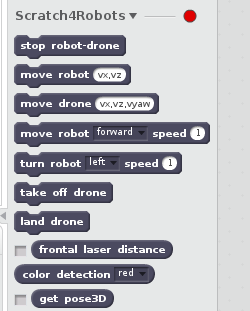
\includegraphics[scale=0.75]{img/bloques-s4r.png}
  	\caption{Bloques propios de la extensión Scratch4Robots}
  	\label{fig:curiosity}
\end{figure}



EXPLICAR LÓGICA DE LOS BLOQUES EN PYTHON

-- explicar los perceptivos

-- explicar el problema con los de movimiento y las listas, solución aportada
